\section{Desarrollo}
\subsection{Hardware}\label{sec:hw}

El prototipo para Smart House está equipado con etapas de potencia de corriente alterna y directa, etapa de adquisición de datos, entre otras características que permitan cumplir con los objetivos planteados. Este fue Diseñado en el software Proteus, desde el esquemático hasta la placa de circuito impreso (PCB), en la figura \ref{fig:esp32} se observa el esquematico de la tarjeta ESP32 construido junto con su distribución de pines, además de sus conexiones correspondientes dentro de este programa. El prototipo está separado en dos secciones, la etapa de potencia AC y la etapa DC, en la última, se encuentra la mayor parte de circuitos que funcionan con corriente directa.\\

%\begin{figure}[H]
%	\centering
%	\caption{ESP32 creado en proteus [Imagen Propia]}
%	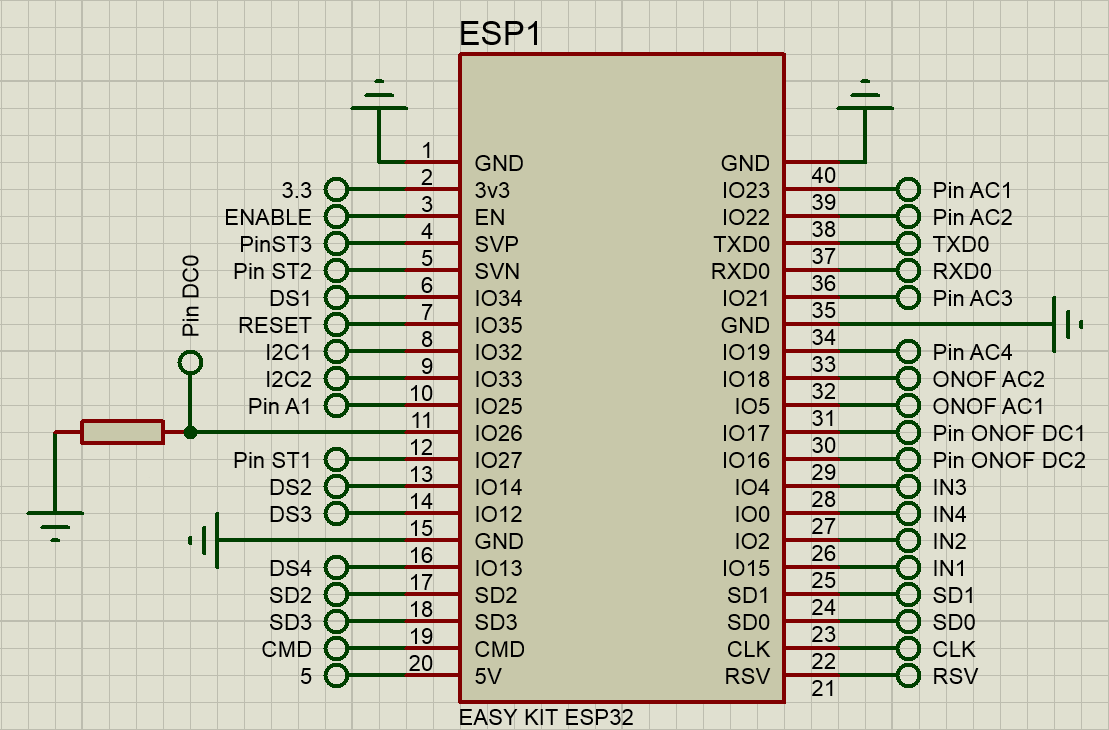
\includegraphics[width=0.5\linewidth]{Imagenes/ESP32}	
%	\label{fig:esp32}
%\end{figure}

En los siguientes ítems se resaltaran las características más importantes que lleva el circuito:\\

	\subsubsection{Alimentacion}
	
	\paragraph{Corriente alterna (AC)}
		El prototipo recibe el voltaje directamente de la red eléctrica a la que se encuentra conectado el entorno de aplicación, para el caso de Colombia, la red doméstica comúnmente otorga 110V AC, los cuales son regulados para el funcionamiento adecuado del prototipo, como la etapa de potencia AC y el detector de cruce por cero con el fin de sincronizar la tarjeta a dicha red eléctrica.\\
		
	\paragraph{Corriente directa (DC)}
		Para la alimentación DC del circuito se hace uso de un conversor AC-DC que regula el voltaje de la red eléctrica a 12V DC y 2A, con los cuales se manejara la etapa de potencia DC, además de ser usados por dos modulos conversores DC-DC, ambos con entradas de 12V DC y con salidas a los niveles lógicos comunes, 5V y 3.3V, empleados con el fin de alimentar dispositivos como opto acopladores, transistores BJT o relevadores con activación de 5V, así como también la tarjeta de prototipo ESP32.\\
			
%		\begin{figure}[H]
%			\centering
%			\caption{Modulo conversor DC-DC. Tomado de: \cite{DCDC}}
%			\label{fig:DCDC}
%			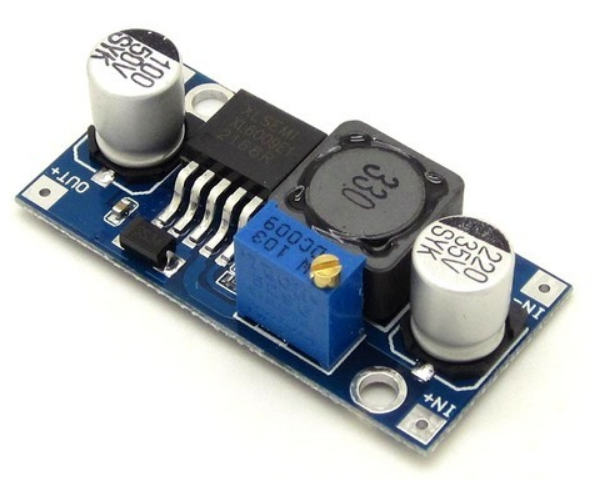
\includegraphics[width=0.5\linewidth]{Imagenes/DCDC}
%		\end{figure}
	
	\subsubsection{Entradas}
	\paragraph{Sensores}
		el prototipo viene equipado con una etapa de adquisición de datos con capacidad entre 7 a 134 sensores, pues posee una entrada I2C, ampliando el número de dispositivos conectados, lo cual también permitiría adicionar tareas más específicas en escenarios que lo requieran.\\
		
	 	Teniendo en cuenta que el ESP32 funciona en voltajes lógicos de 3.3V, se tienen 4 entradas de sensores directamente conectados a los pines de la tarjeta, con la capacidad de cambiar el voltaje de alimentación para 3 de ellos, pues en el mercado se encuentran sensores que manejan voltajes de alimentación ya sea de 3.3V o 5V, mientras que la cuarta entrada se encuentra alimentada con 5V para un sensor analogico, esta viene acondicionada con un diodo zener en contraposición, para evitar que la tarjeta ESP32 tenga un voltaje de entrada superior a 3.3V.\\
		
		Las tres entradas para sensores de estado, a diferencia de las demás, se encuentran conectadas a pines de la tarjeta que no presentan resistencia de pull down por software, por ello se agregan estas dentro del hardware del sistema.\\
		
%		\begin{figure}[H]
%			\centering
%			\caption{Entrada de sensores[Imagen Propia]}
%			\label{fig:SVS}
%			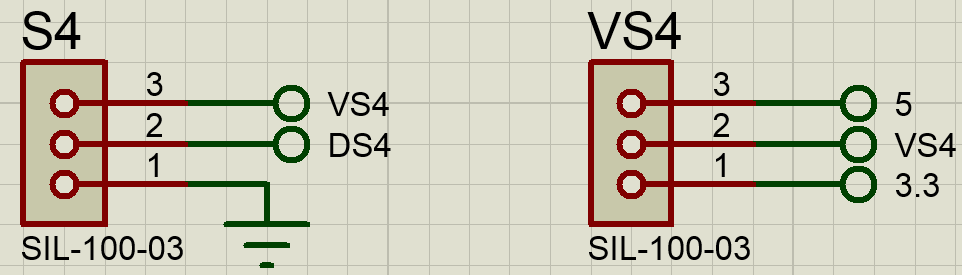
\includegraphics[width=0.7\linewidth]{Imagenes/SVS}
%		\end{figure}
%	
%		\begin{figure}[H]
%			\centering
%			\caption{Entrada para sensor de calidad de aire[Imagen Propia]}
%			\label{fig:S1Aire}
%			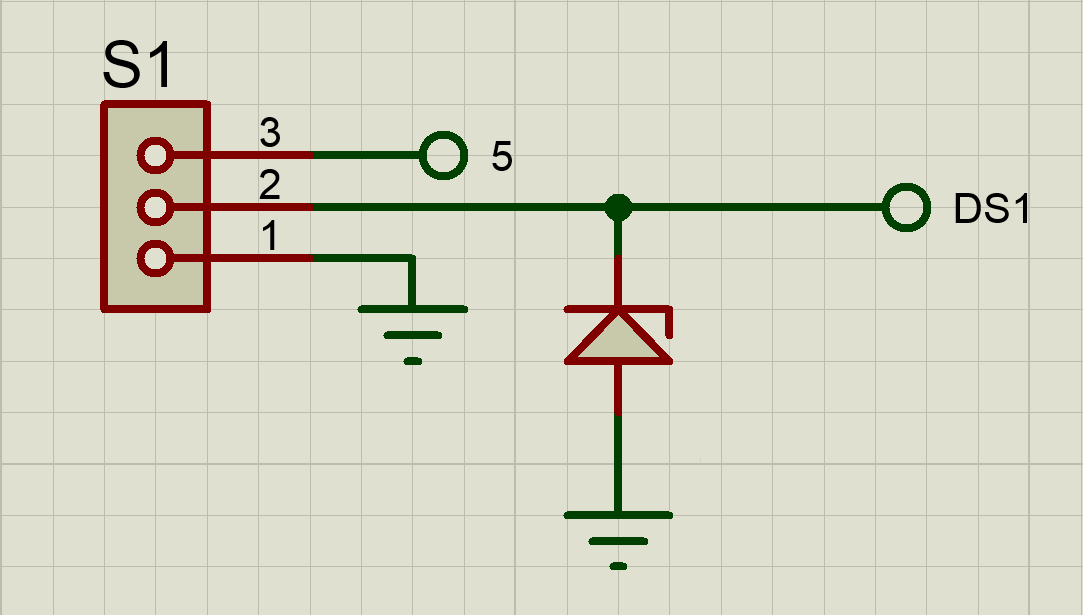
\includegraphics[width=0.6\linewidth]{Imagenes/S1Aire}
%		\end{figure}
%	
%		\begin{figure}[H]
%			\centering
%			\caption{Entrada para sensores con resistencia de pull down[Imagen Propia]}
%			\label{fig:ST}
%			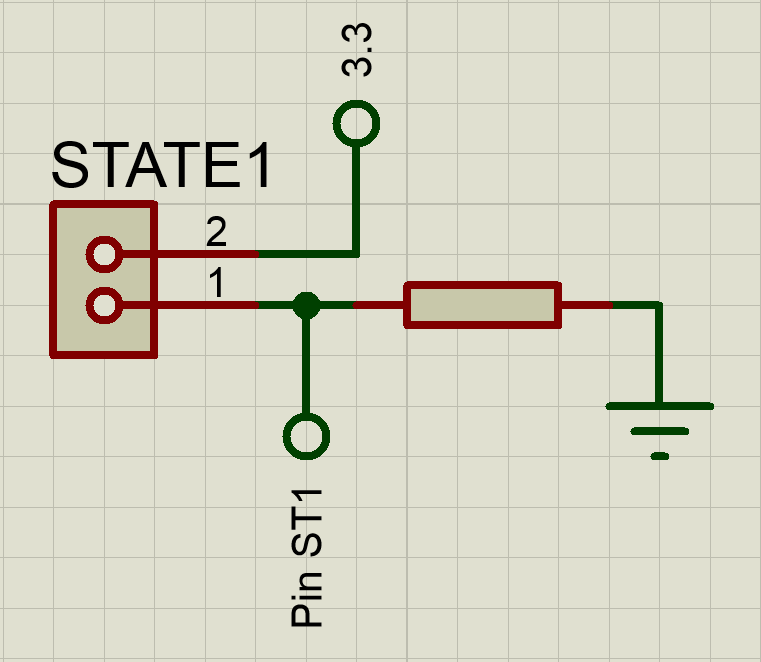
\includegraphics[width=0.5\linewidth]{Imagenes/ST}
%		\end{figure}		
	
	\paragraph{Interacción con el sistema}
		Para calibrar la salida audible se hace uso de una resistencia variable (Potenciometro), el cual permite regular el voltaje de entrada al circuito de amplificación que será descrito en el presente capitulo en la sección de salidas del hardware.\\
		
		Presionando el botón enable se reinicia la tarjeta ESP32, junto con su firmware.\\
		
		Presionando el botón reset se borran las credenciales ingresadas para la conexión del ESP32 a la red wifi.\\
	
		
	\subsubsection{Salidas:}
	\paragraph{Etapa de potencia AC}
		Se encuentra diseñada a una potencia de 2000W en un total de seis cargas, cuatro de ellas cuentan con un circuito para el control por ángulo de fase, como se observa en la figura \ref{fig:CAC1}, con una capacidad individual de 500W, gracias a el TRIAC BTA26600, el cual soporta una corriente máxima de 25A; con el fin de proteger el ESP32, se hace uso de optoacopladores MOC3021, debido a su funcionalidad de aislar circuitos de forma óptica.\\
		
%		\begin{figure}[H]
%			\centering
%			\caption{Control por angulo de fase [Imagen Propia]}
%			\label{fig:CAC1}
%			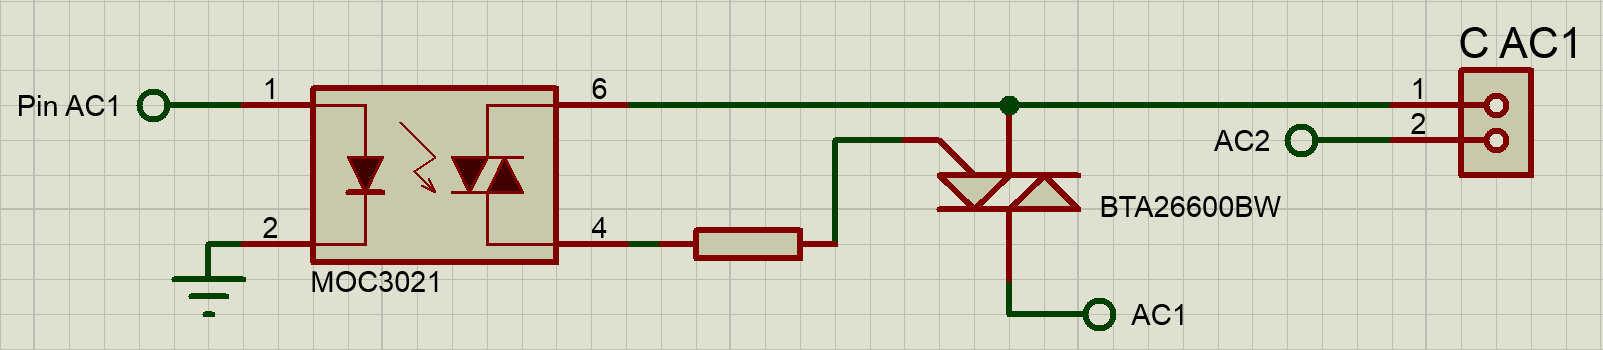
\includegraphics[width=0.8\linewidth]{Imagenes/CAC1}
%		\end{figure}
%	
%		\begin{figure}[H]
%			\centering
%			\caption{Triac BTA26600. Tomado de: \cite{TRIAC}}
%			\label{fig:TRIAC}
%			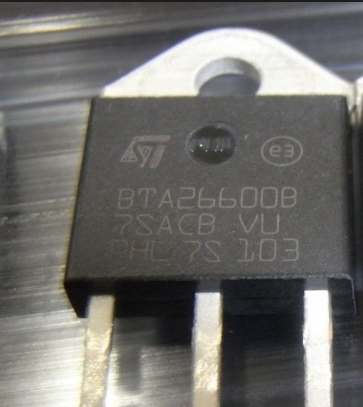
\includegraphics[width=0.35\linewidth]{Imagenes/TRIAC}
%		\end{figure}
%	
		Las dos cargas restantes corresponden a un sistema de encendido y apagado, cuyo funcionamiento se basa en un relevador SRA-05VDC-CL activado a 5V por medio de un transistor BJT como switch, gracias a este relé, las salidas tienen capacidad de hasta 200W cada una, en la figura \ref{fig:ONOFAC} se observa el circuito diseñado en proteus. Para proteger el ESP32 el prototipo se vale de ese dispositivo, puesto que presenta un aislamiento magnético por la naturaleza de su operación.\\
	
%		\begin{figure}[H]
%			\centering
%			\caption{Interruptor para cargas AC [Imagen Propia]}
%			\label{fig:ONOFAC}
%			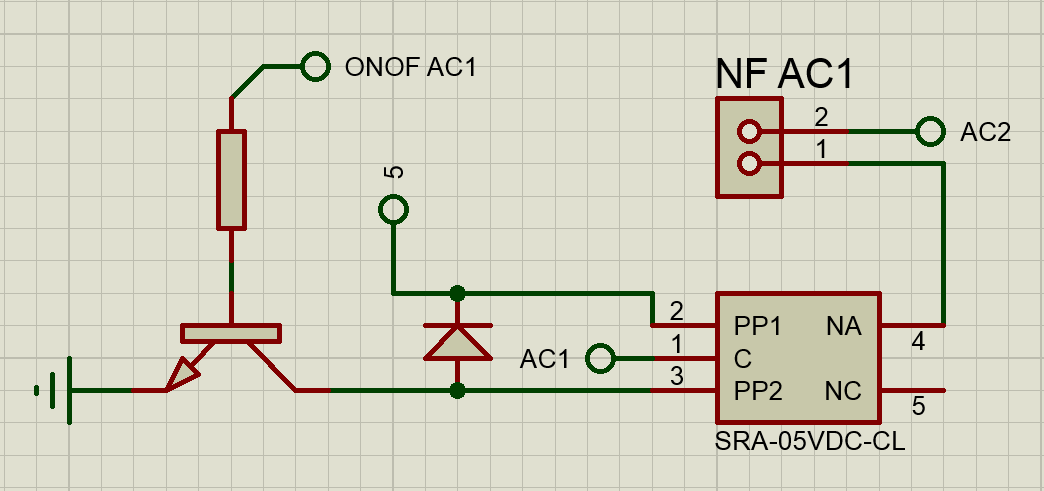
\includegraphics[width=0.7\linewidth]{Imagenes/ONOFAC}
%		\end{figure}
	
		Dentro de la etapa AC se encuentra el detector de cruce por cero, el cual se vale de un fototransistor 4N25, debido a su alta capacidad de aislamiento, tomando la onda rectificada completa y pasándola a un nivel lógico de 3.3V, esta parte del circuito se observa en la figura \ref{fig:DC01}; para que la señal sea más confiable se hace uso de un Schmitt-Trigger CD40106 mostrado en la figura \ref{fig:DC02}, valiéndose de la histéresis de voltaje garantizando que la señal de salida sea poco susceptible al ruido \cite{DC0}.\\
		
%		\begin{figure}[H]
%			\centering
%			\caption{Detector de cruce por cero [Imagen Propia]}
%			\label{fig:DC01}
%			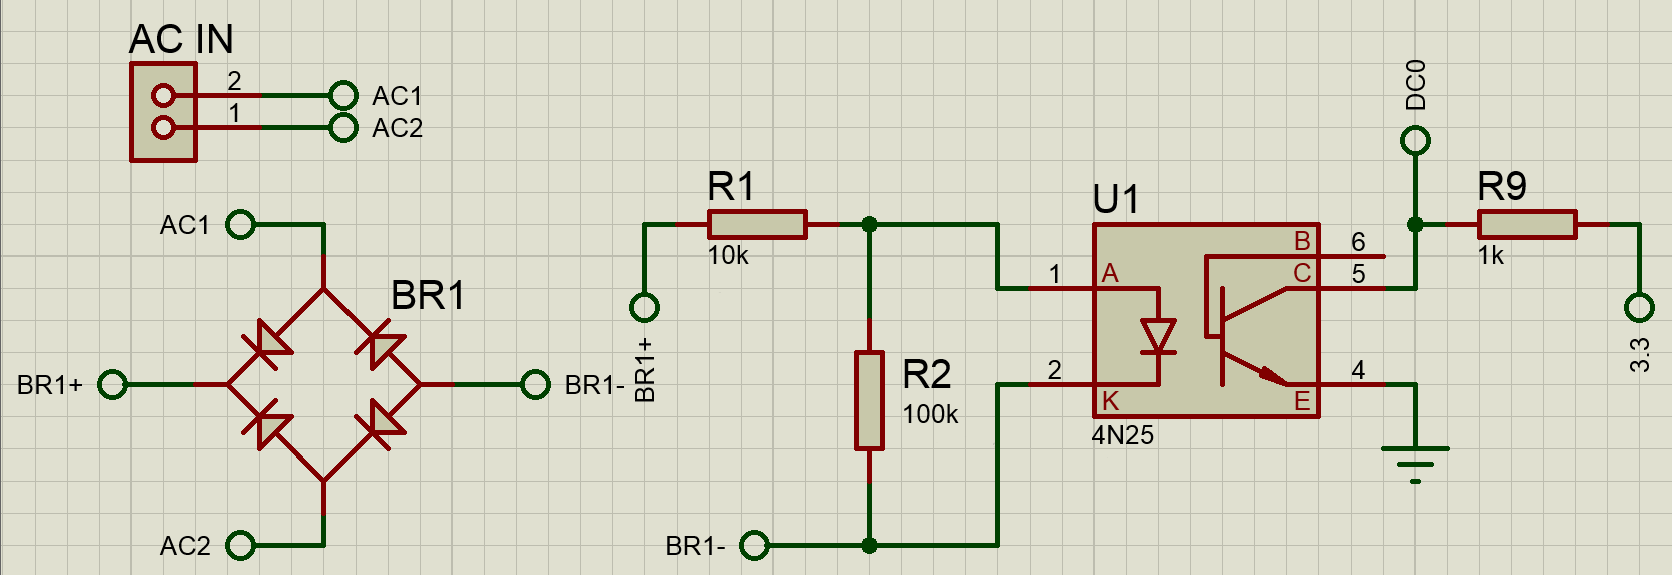
\includegraphics[width=0.85\linewidth]{Imagenes/DC01}
%		\end{figure}
%	
%		\begin{figure}[H]
%			\centering
%			\caption{Schmitt trigger para el detector de cruce por cero [Imagen Propia]}
%			\label{fig:DC02}
%			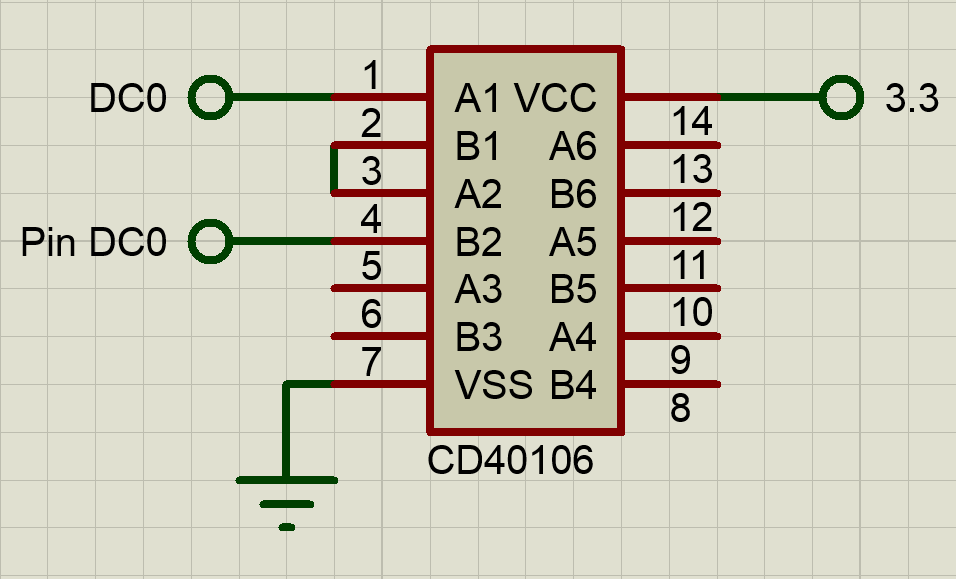
\includegraphics[width=0.5\linewidth]{Imagenes/DC02}
%		\end{figure}
	
	\paragraph{Etapa DC}
		esta etapa cuenta con cuatro salidas de control diseñadas para cargas de 12V, de las cuales, dos de ellas tienen un enfoque enfoque a motores, puesto que está equipada con control de velocidad a base de PWM e inversión de giro con un puente h usando transistores mosfet IRLZ44N; el puente h se encuentra controlado por un circuito integrado L293D, que garantiza un voltaje Vgs adecuado para la correcta activación del los transistores del puente h; este circuito se muestra en la figura \ref{fig:L293D} y \ref{fig:CDC}.\cite{IRL}.\\
		
		Las dos salidas restantes también cuentan con mosfet IRLZ44N, y su control igualmente es a base de PWM, mas no permite realizar la inversión de giro, por lo cual se enfoca a dispositivos como lámparas LEDs, el diseño en proteus se muestra en la figura \ref{fig:ONOFDC}.\\
		
%		\begin{figure}[H]
%			\centering
%			\caption{Integrado L293D [Imagen Propia]}
%			\label{fig:L293D}
%			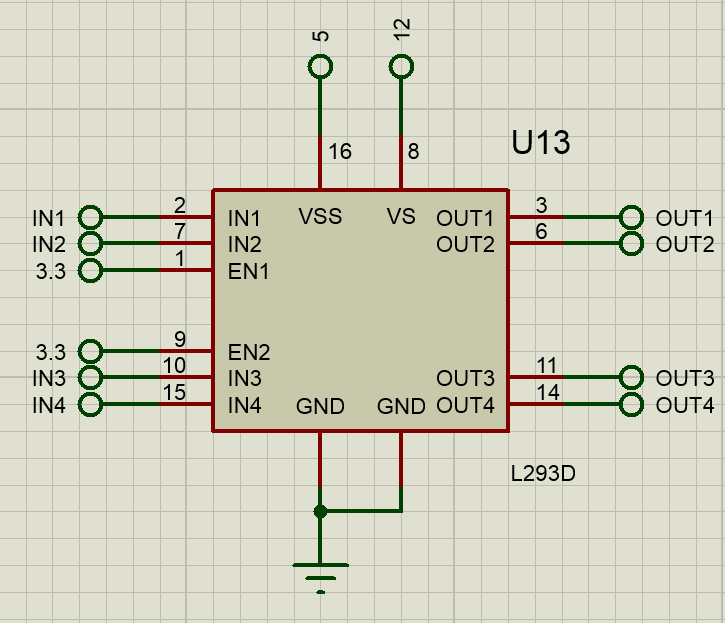
\includegraphics[width=0.5\linewidth]{Imagenes/L293D}
%		\end{figure}
%		
%		\begin{figure}[H]
%			\centering
%			\caption{Puente h para control de motores DC [Imagen Propia]}
%			\label{fig:CDC}
%			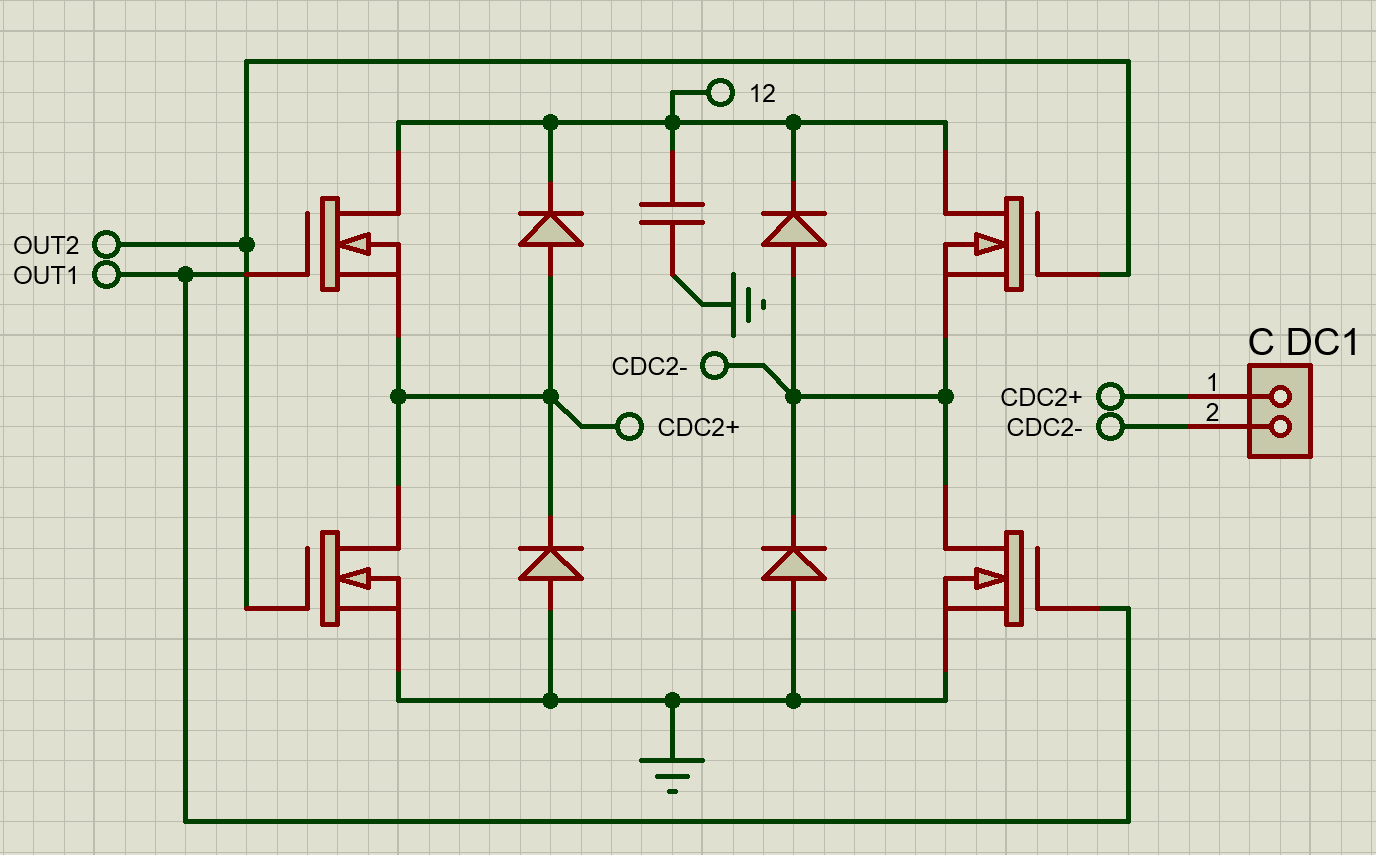
\includegraphics[width=0.7\linewidth]{Imagenes/CDC}
%		\end{figure}
%	
%		\begin{figure}[H]
%			\centering
%			\caption{Control para cargas DC [Imagen Propia]}
%			\label{fig:ONOFDC}
%			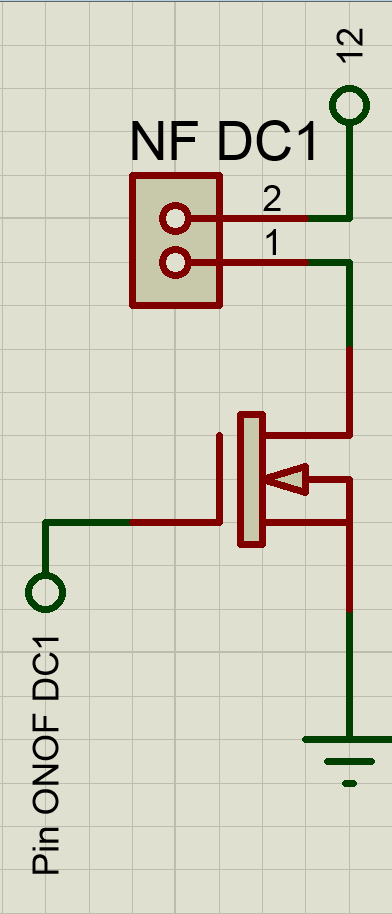
\includegraphics[width=0.25\linewidth]{Imagenes/ONOFDC}
%		\end{figure}
	
	\paragraph{Salida audible}
		está diseñada para emitir desde sonidos a una sola frecuencia, o sonido mono estéreo, caso dado cuando se activa una regla programada en la aplicación web, enfocada a las cargas de encendido y apagado, tanto de la etapa de potencia AC como la etapa DC; el sonido emitido por el prototipo corresponde a una voz con tonalidad femenina, pronunciando el estado en el cual se configura la carga según la regla (ya sea encendido, o apagado).\\
		
		El circuito utilizado para la salida audible está basado en el amplificador de audio LM386, implementando el esquema típico de aplicación ilustrado en su datasheet \cite{LM386}, en la figura \ref{fig:AUD} se observa implementado en el software proteus.
		
		
%		\begin{figure}[H]
%			\centering
%			\caption{Circuito tipico para el LM386 [Imagen Propia]}
%			\label{fig:AUD}
%			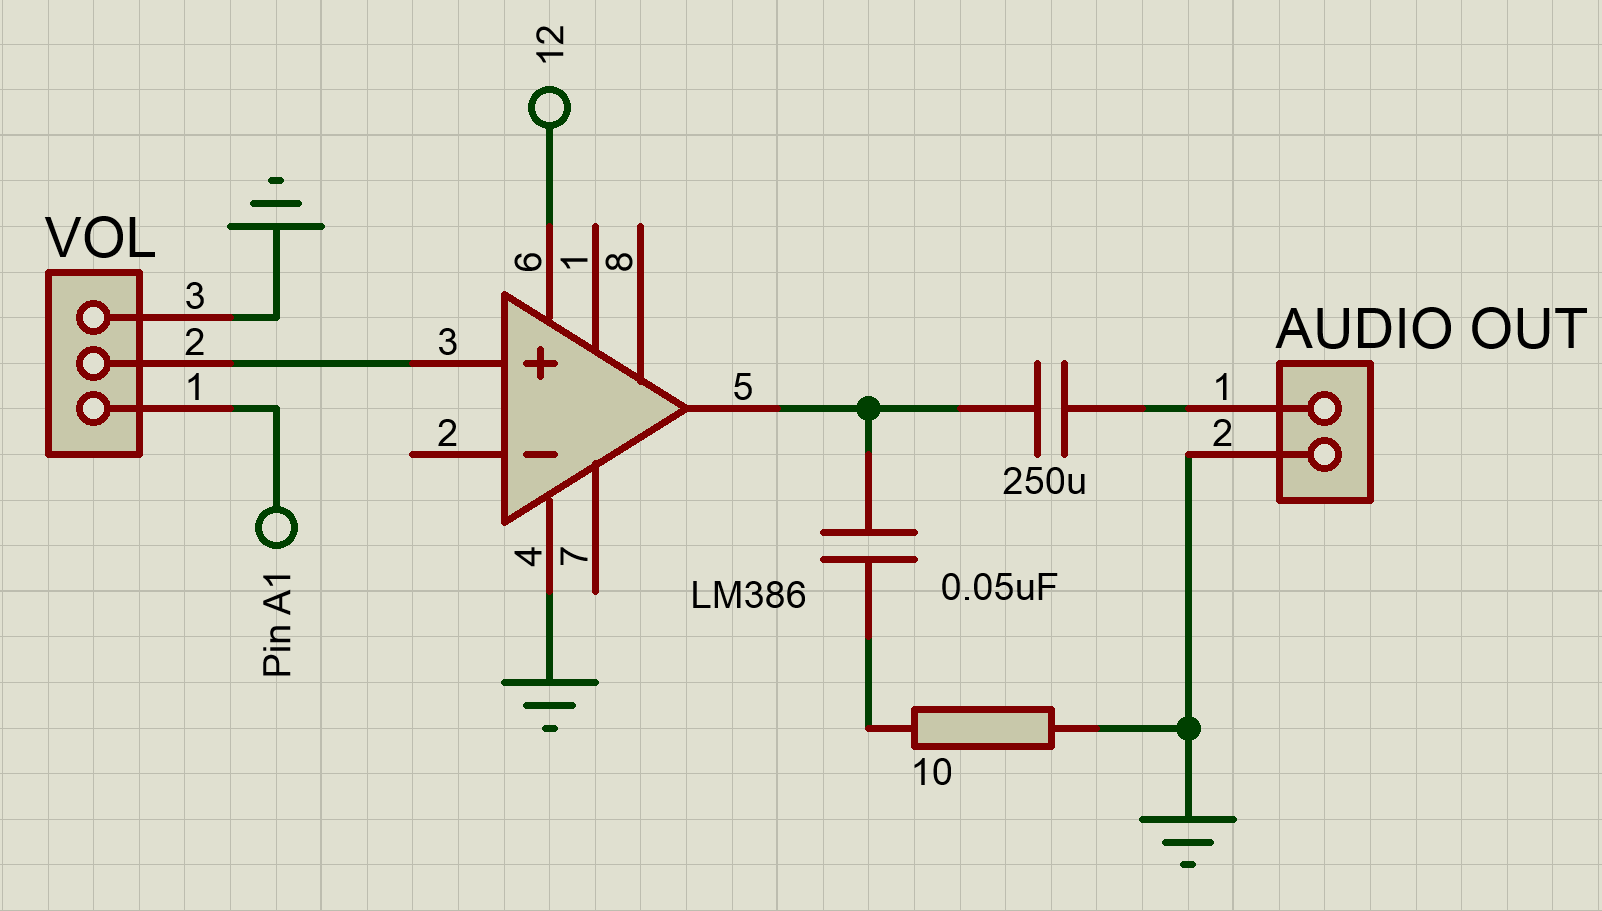
\includegraphics[width=0.7\linewidth]{Imagenes/AUD}
%		\end{figure}		
				
\subsection{Firmware}

El firmware se desarrolla sobre el framework o SDK oficial de Espressif Systems, ESP-IDF el cual posee una documentación \cite{ES} muy útil a la hora de utilizar las diferentes APIs presentes en este; para el desarrollo de la aplicación es necesario contar con los requisitos que se observan en la figura \ref{fig:what-you-need}. El framework incluye un kernel de tiempo real llamado FreeRTOS, el cual da soporte al manejo de los diversos recursos del sistema; al ser un RTOS, las funciones se definen mediante tareas, entonces cada funcionalidad de la tarjeta o grupo de funcionalidades se desarrolla en una o varias tareas que realicen las acciones adecuadas.

%\begin{figure}[H]
%	\centering
%	\caption{ESP-IDF. Tomado de: \cite{ES}}
%	\label{fig:what-you-need}
%	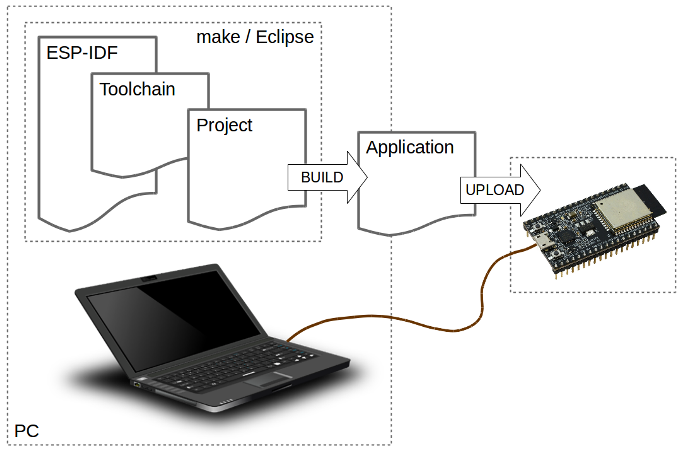
\includegraphics[width=0.5\linewidth]{Imagenes/what-you-need}
%\end{figure}

\subsection{Software}

En esta sección se desarrolla una aplicación web, la cual se encarga de ejecutar la gestión entre el usuario y la tarjeta. De este modo, se usa un patrón de arquitectura Modelo-Vista-Controlador (MVC). Aquel modelo es realmente útil ya que separa la lógica de negocio de la interfaz de usuario, incrementando la reutilización y flexibilidad, además la escalabilidad de ambos aspectos por separado, dicho esto la aplicación cuenta con diferentes modelos, controladores y vistas \cite{MVC1}. La función de cada parte de esta arquitectura se puede observar en la figura \ref{fig:mvc}.\\

%\begin{figure}[H]
%	\centering
%	\caption{Modelo-Vista-Controlador [Imagen Propia]}
%	\label{fig:mvc}
%	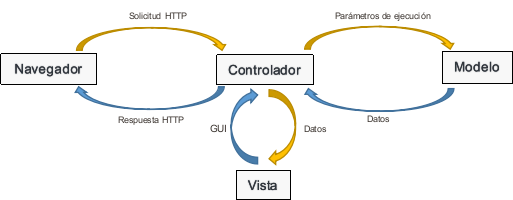
\includegraphics[width=0.7\linewidth]{Imagenes/MVC}
%\end{figure}

Además, con este framework se hace uso de un ORM (Mapeo Objeto-Relacional) llamado Eloquent. Esta es una forma de mapear los datos que se encuentran en la base de datos a objetos de PHP y viceversa, esto facilita el uso de diferentes gestores de bases de datos como MySQL, SQLite, entre otras, ya que todas las consultas estan en PHP y el ORM ya se encarga del mapeo a los comandos SQL como se observa en la figura \ref{fig:orm}. Eloquent usa los modelos para enviar y recibir información de la base de datos\cite{Eloq}.

%\begin{figure}[H]
%	\centering
%	\caption[ORM]{ORM [Imagen Propia]}
%	\label{fig:orm}
%	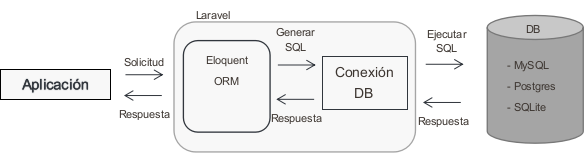
\includegraphics[width=0.7\linewidth]{Imagenes/ORM}
%\end{figure}

\subsection{Prueba Beta}

Esta prueba se desarrolla en el entorno del cliente o usuario, arrojando resultados sobre las funcionalidades provistas para el software, además de dar la aceptación por parte del cliente si el producto funciona de manera adecuada o esperada \cite{PB}. Con el fin de realizar dicha vereficación se analizan los objetivos a cumplir y los alcances, por lo tanto se separan los casos de prueba con el propósito de formular las preguntas que deben contestar las personas. las preguntas formuladas para estos se encuentran en el Anexo \ref{AnexoB}.\\

\paragraph{Prueba de conectividad de la tarjeta:} en la cual la persona que participa en esta prueba debe realizar los primeros pasos para conectar la tarjeta con internet como se expone más adelante en resultados y se explica en Anexos en el manual de usuario.\\

\paragraph{Prueba de la Aplicación Web:} en la cual se evalúan diferentes aspectos y la mas extensa, ya que se evalúa el inicio de sesión, el monitoreo y control de todos los dispositivos que se encuentra conectados en tarjeta SmartHouse, además de las funcionalidades que posee el sistema en general.